\documentclass{beeper}

\usepackage{fontawesome}
\usepackage{etoolbox}
\usepackage{textcomp}
\usepackage[nodisplayskipstretch]{setspace}
\usepackage{xspace}
\usepackage{verbatim}
\usepackage{multicol}
\usepackage{soul}
\usepackage{attrib}

\usepackage{amsmath,amssymb,amsthm}

\usepackage[linesnumbered,commentsnumbered,ruled,vlined]{algorithm2e}
\newcommand\mycommfont[1]{\footnotesize\ttfamily\textcolor{blue}{#1}}
\SetCommentSty{mycommfont}
\SetKwComment{tcc}{ \# }{}
\SetKwComment{tcp}{ \# }{}

\usepackage{siunitx}

\usepackage{tikz}
\usepackage{pgfplots}
\usetikzlibrary{decorations.pathreplacing,calc,arrows.meta,shapes,graphs}

\AtBeginEnvironment{minted}{\singlespacing\fontsize{10}{10}\selectfont}
\setmainfont{Open Sans Light}
\usefonttheme{serif}

\makeatletter
\patchcmd{\beamer@sectionintoc}{\vskip1.5em}{\vskip0.5em}{}{}
\makeatother

% Math stuffs
\newcommand{\Z}{\mathbb{Z}}
\newcommand{\R}{\mathbb{R}}
\newcommand{\N}{\mathbb{N}}
\newcommand{\lcm}{\text{lcm}}
\newcommand{\Inn}{\text{Inn}}
\newcommand{\Aut}{\text{Aut}}
\newcommand{\Ker}{\text{Ker}\ }
\newcommand{\la}{\langle}
\newcommand{\ra}{\rangle}

\newcommand{\yournewcommand}[2]{Something #1, and #2}

\newenvironment{question}[1]{\par\textbf{Question #1.}\par}{}

\newcommand{\pmidg}[1]{\parbox{\widthof{#1}}{#1}}
\newcommand{\splitslide}[4]{
    \noindent
    \begin{minipage}{#1 \textwidth - #2 }
        #3
    \end{minipage}%
    \hspace{ \dimexpr #2 * 2 \relax }%
    \begin{minipage}{\textwidth - #1 \textwidth - #2 }
        #4
    \end{minipage}
}

\newcommand{\frameoutput}[1]{\frame{\colorbox{white}{#1}}}

\newcommand{\tikzmark}[1]{%
\tikz[baseline=-0.55ex,overlay,remember picture] \node[inner sep=0pt,] (#1)
{\vphantom{T}};
}

\newcommand{\braced}[3]{%
    \begin{tikzpicture}[overlay,remember picture]
        \draw [thick,decorate,decoration={brace,raise=1ex,amplitude=4pt},blue] (#2.south west-|T1.south west) -- node[anchor=west,left,xshift=-1.8ex,text=olive]{#3} (#1.north west-|T1.south west);
    \end{tikzpicture}
}

\title{Architecting for Scale}
\subtitle{A case-study in utilizing a sharded architecture for infinite* scalability}
\author{Sumner Evans}
\institute{Beeper}
\date{27 September 2022}

\begin{document}

\begin{frame}{A bit about me}
    My name is Sumner, I'm a \textbf{software engineer at Beeper}.
    \begin{itemize}
        \item I graduated from Colorado School of Mines in 2018 with my
            bachelor's in CS and 2019 with a master's in CS.
        \item I am an adjunct professor. Currently I'm teaching CSCI 400. I've
            taught 406, and 564 in the past as well.
        \item I enjoy skiing, volleyball, and soccer.
        \item I'm a 4th degree black belt in ATA taekwondo.
    \end{itemize}
\end{frame}

\begin{frame}{Overview}
    \setbeamertemplate{section in toc}[sections numbered]
    \tableofcontents[hideallsubsections]

    \begin{block}{This talk is interactive!}
        If you have questions at any point, feel free to interrupt me.
    \end{block}
\end{frame}

\section{A bit about Beeper}

\begin{frame}{Beeper's mission}
    Our mission is to:\\

    \begin{quote}
        make it easy for everyone on Earth to chat with each other.
    \end{quote}
    \pause

    We specifically chose the word ``chat'' rather than ``communicate'' because
    we are focusing on \textit{people talking to one another}.
\end{frame}

\begin{frame}{What is Beeper?}
    \begin{center}
        \textbf{Beeper is an app that brings all of your chat networks together into
            a single inbox.}
    \end{center}
    \centerline{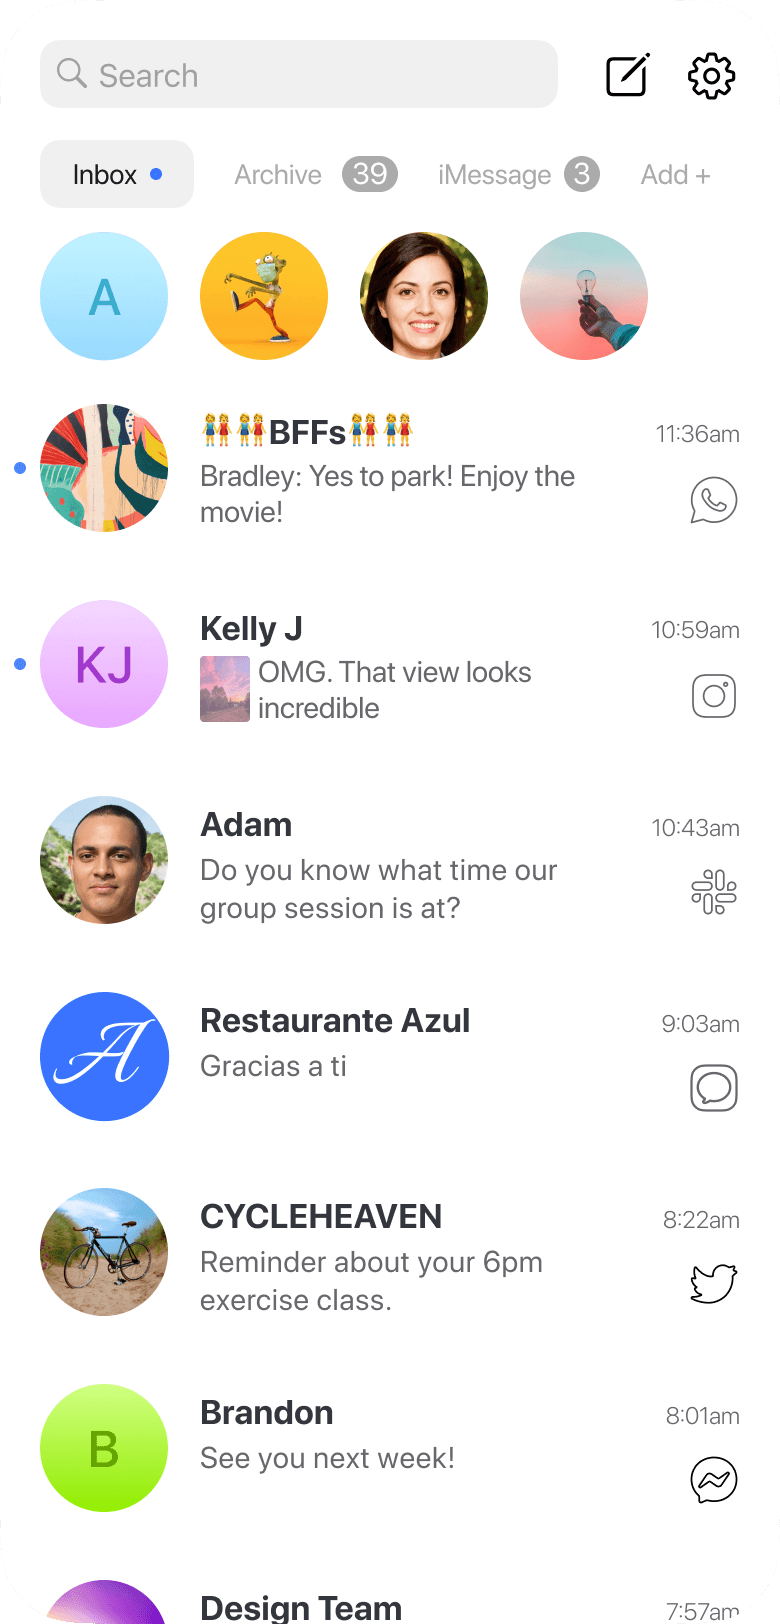
\includegraphics[width=0.3\textwidth]{images/beeper-mobile}}
\end{frame}

\begin{frame}{What is Beeper?}
    \textbf{Beeper allows you to consolidate messages from 15+ chat apps into a
        single inbox.}

    \pause
    \begin{itemize}
        \item Beeper is available on on macOS, Windows, Linux iPhone, iPad,
            Android and Chrome OS.
        \item Beeper is built on top of the Matrix protocol.
        \item Beeper encrypts all chats, including bridged chats, by
            default\footnote[frame]{We have to momentarily decrypt your chat
            messages to translate from the other network to Matrix, but we never
            log or store your unencrypted messages.}.
    \end{itemize}
\end{frame}

\begin{frame}{We are targeting individuals, not enterprises}
    \begin{center}
        \textbf{\Large We want to beat WhatsApp, not Slack.}
        \vspace{1cm}
        \pause

        \textbf{\large Our core competency is the 50th highest priority at the
        big tech companies.}

        Most chat networks are an afterthought within the ecosystem of a larger
        company. At Beeper, chat is all we care about.
    \end{center}
\end{frame}

\begin{frame}{How we make money}
    \textbf{We charge a flat \$10/month fee to use Beeper.} This fee allows
    users to connect as many chat networks as they want.
    \pause

    \textbf{No ads. No data mining.} We take advantage of Matrix's E2EE to add
    additional privacy guarantees.
    \pause

    \begin{center}
        \LARGE
        \textbf{The transaction is simple:\\ users pay us money for a service.}
    \end{center}
\end{frame}

\begin{frame}{Bridging to a glorious Matrix future}
    We see bridges as a way to onboard users into the Matrix ecosystem.

    Users can switch to a new app without loosing a single conversation!
    \pause

    \vspace{1cm}
    \begin{center}
        \Large
        \textbf{We encourage our users to connect \textit{all} of their chat
        networks to Beeper.}
    \end{center}
\end{frame}

\section{What we've built}

\begin{frame}{Custom clients for desktop and mobile}
    We forked Element, and added custom features.
    \vspace{0.5cm}

    \centerline{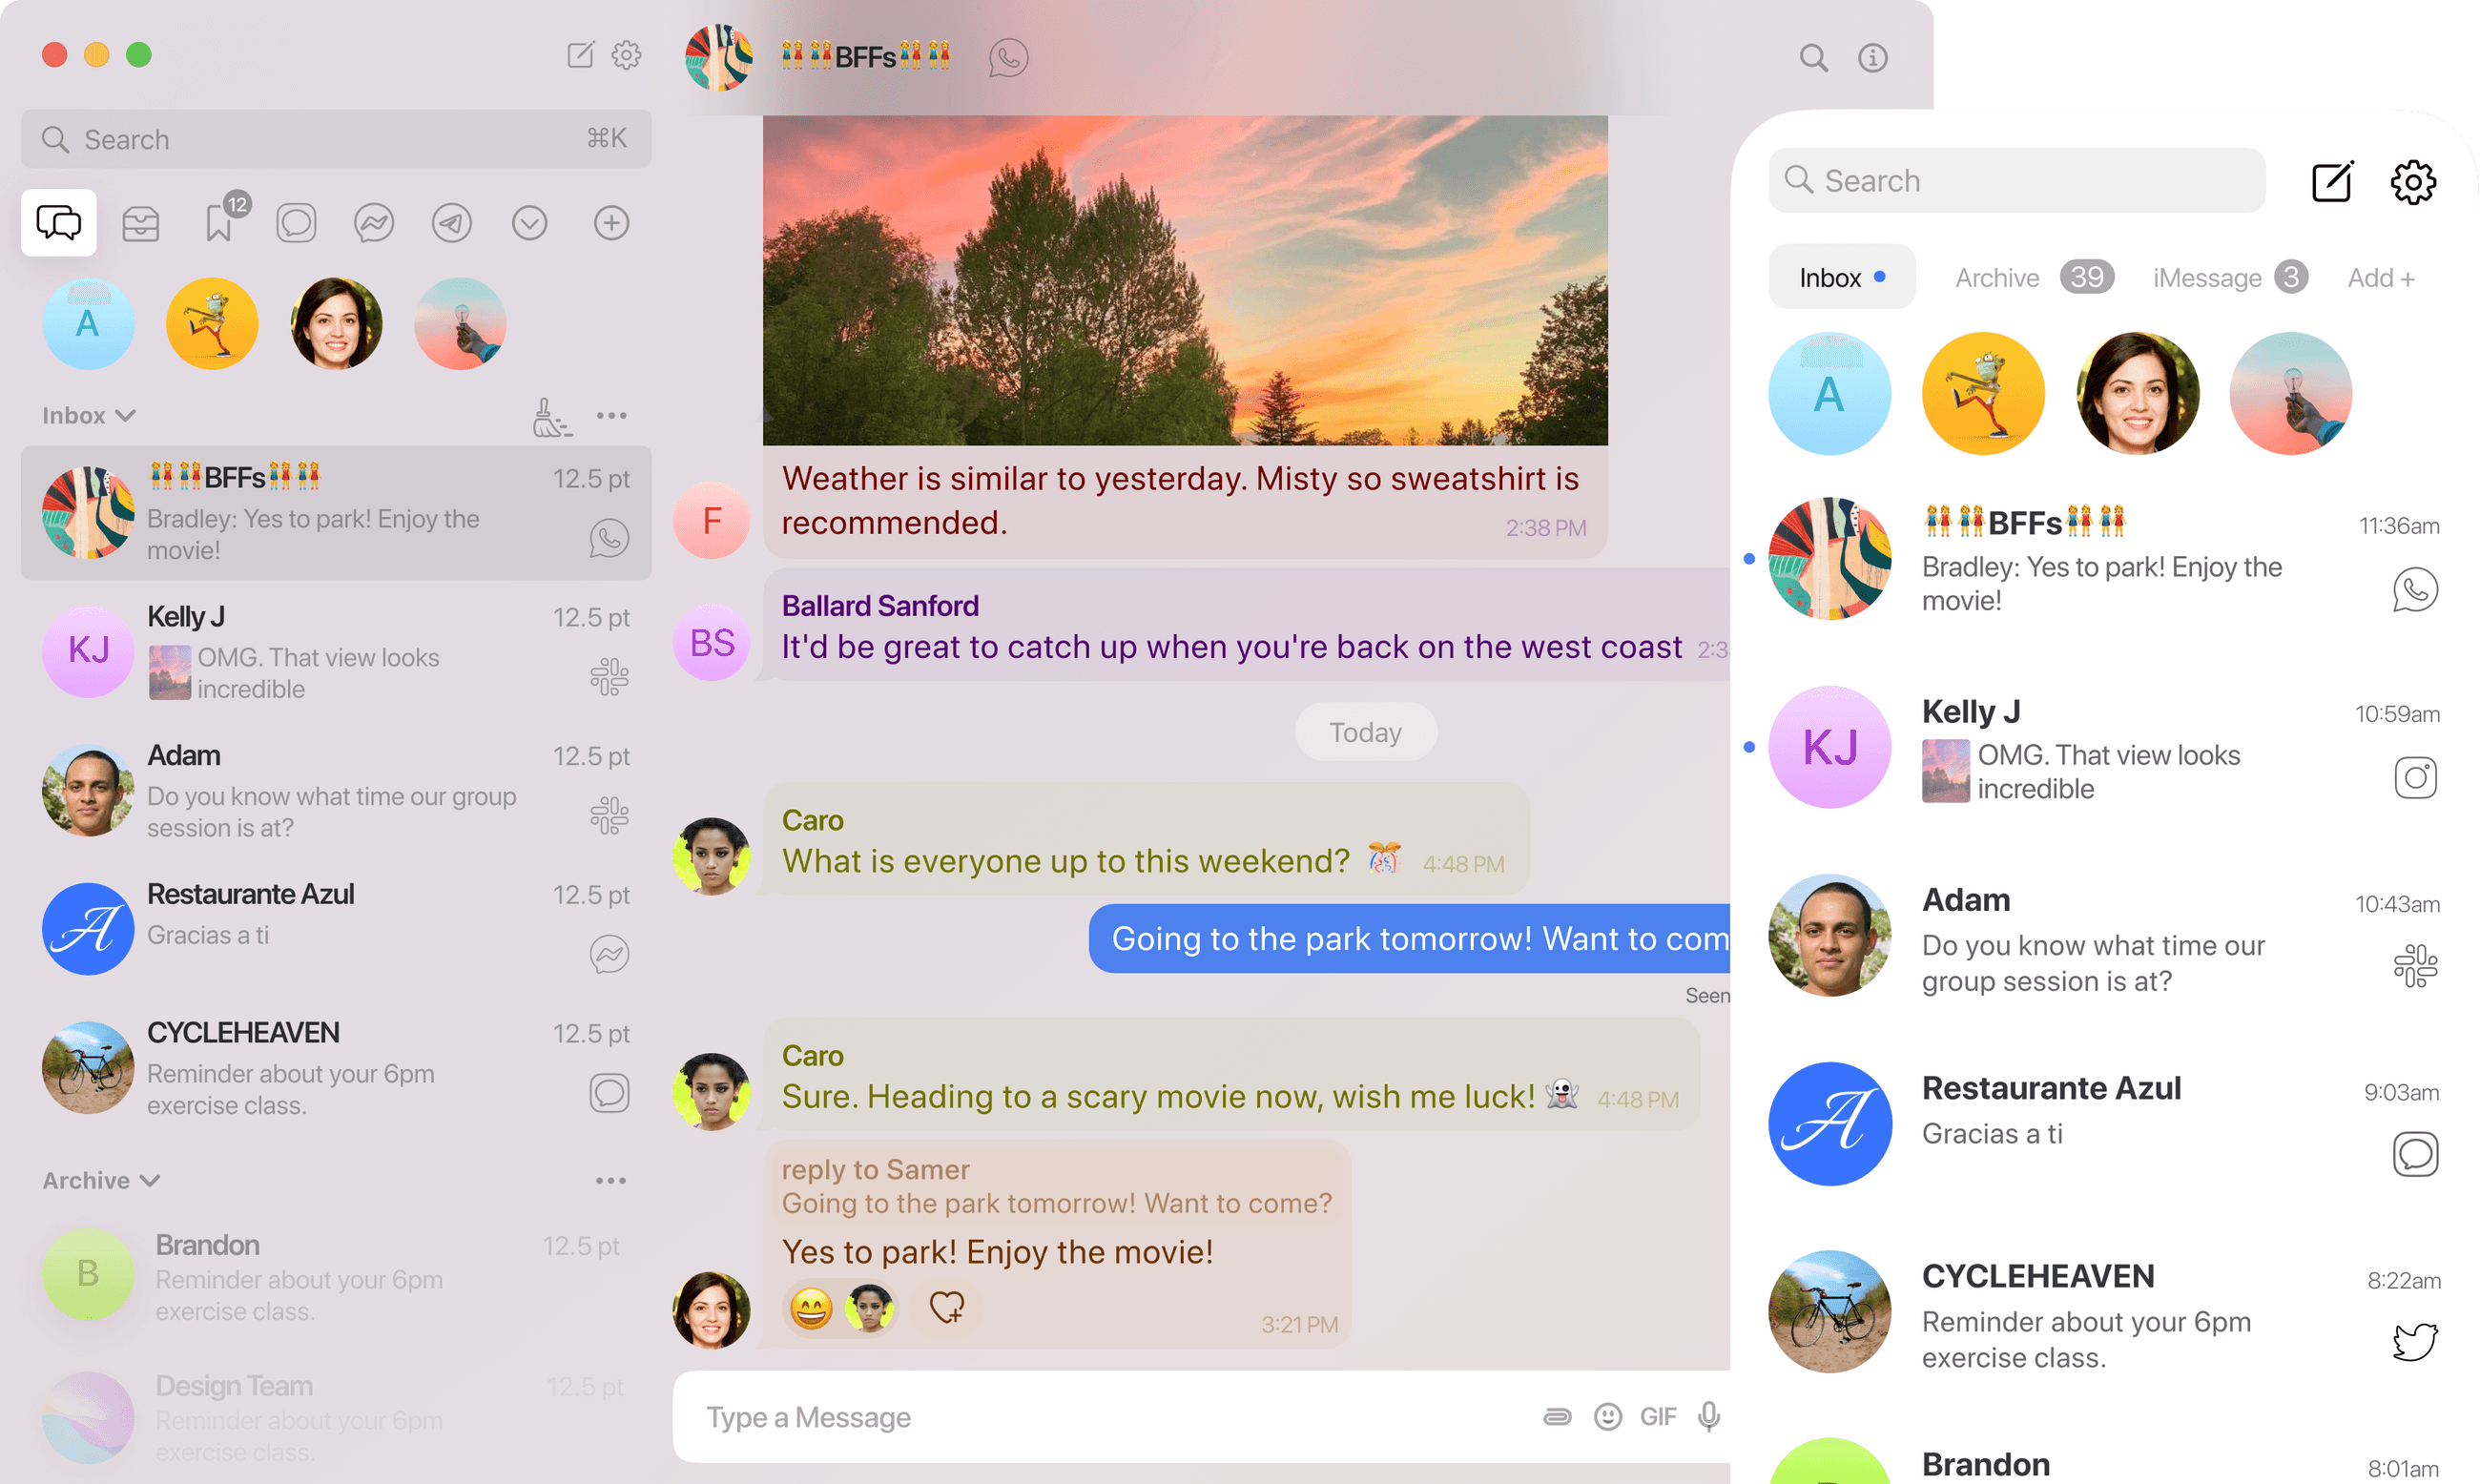
\includegraphics[width=\textwidth]{images/desktop-and-mobile}}
\end{frame}

\begin{frame}{Bridges, bridges, and more bridges!}
    We have built bridges to 10 networks:
    \begin{multicols}{2}
        \begin{itemize}
            \item iMessage
            \item WhatsApp
            \item Facebook Messenger
            \item SMS (Android)
            \item Telegram
            \item Signal
            \item LinkedIn
            \item Instagram
            \item Twitter
            \item Google Chat
        \end{itemize}
    \end{multicols}

    \pause
    We are actively developing new bridges to Discord and Slack.

    \pause
    You can also connect to IRC (via the Libera.chat bridge) and the rest of the
    Matrix federation.
\end{frame}

\begin{frame}{What I work on at Beeper}
    I am on the newly created \textit{Scaling} team.

    Our current objective is to prepare Beeper for rocket-ship growth.
    \vspace{0.5cm}
    \pause

    I was previously part of the \textit{Bridges} team. 

    Notable projects included:
    \begin{itemize}
        \item Writing the LinkedIn bridge
        \item Adding bridge status reporting and message send status
        \item Implementing massive stability improvements in the Signal bridge
        \item Implementing incremental infinite backfill in our WhatsApp and
            Facebook bridges
    \end{itemize}
\end{frame}

\section{What is software architecture?}

\begin{frame}{What do you think software architecture is?}
    \begin{itemize}[<+->]
        \item What questions do software architects ask?
        \item What concerns do software architects have to take into account?
        \item What tradeoffs do software architects have to consider?
    \end{itemize}
\end{frame}

\begin{frame}{Software architecture is about component interactions}
    \centerline{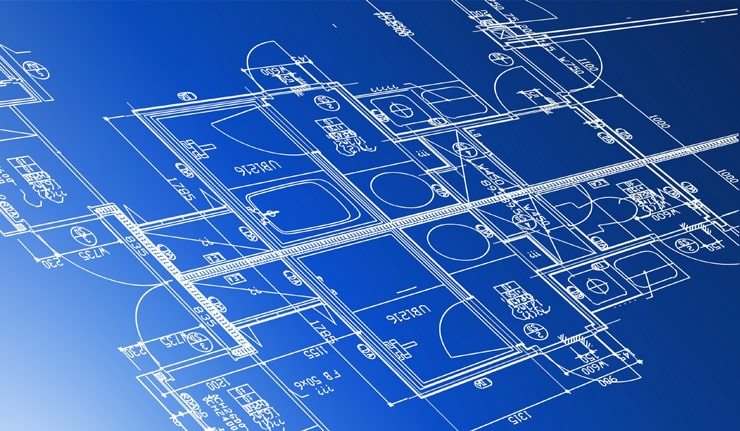
\includegraphics[width=0.7\textwidth]{images/architectural-blueprint}}

    Just like architects have to think about the interactions between plumbing,
    electrical, HVAC, etc., software architects have to think about the
    interactions of components in the software system.
\end{frame}

\begin{frame}{Examples}
    \begin{itemize}[<+->]
        \item 
    \end{itemize}
\end{frame}

\begin{frame}{``The stack''}
    No, not the one you learn in Data Structures.

    \pause

    In software architecture, when we refer to the stack we are referring to the
    tools, services, and languages used for the various components of the
    system.

    The closer a system is to a user, the further \textit{up} the stack it is.
\end{frame}

\section{A bit about Beeper's current architecture}

\begin{frame}{A diagram}
    \centerline{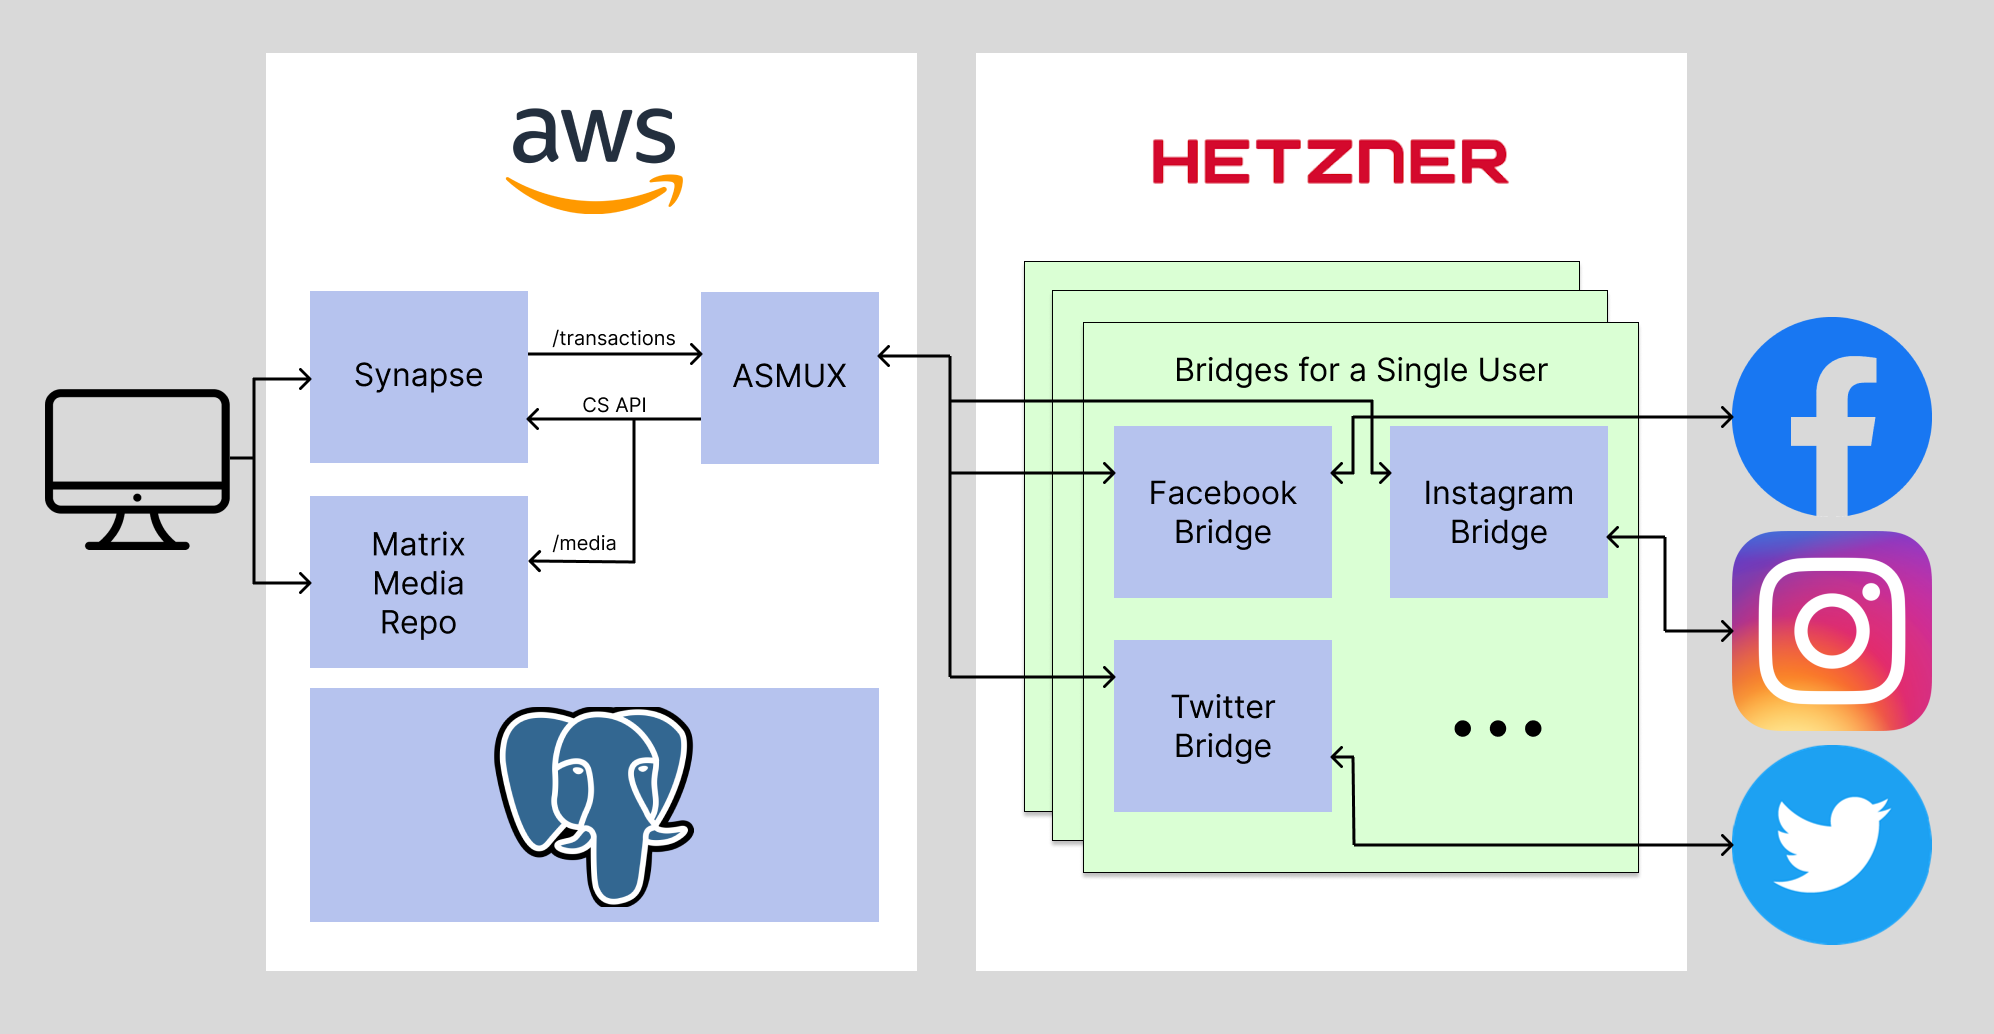
\includegraphics[width=1.15\textwidth]{images/current-architecture}}

    Each user gets their own bridge for each network they connect.
\end{frame}

\begin{frame}{Advantages of our architecture}
    \begin{itemize}[<+->]
        \item ASMUX allows us to dynamically change what bridges are running
        \item Each users' bridge is \textbf{isolated}
        \item We can deploy \textbf{different bridge versions} to different sets
            of users
        \item Bridges can be stopped and started individually
        \item Double puppeting
    \end{itemize}
\end{frame}

\begin{frame}{Disadvantages of our architecture}
    \begin{itemize}[<+->]
        \item We have to run a \textbf{lot} of bridges
        \item Synapse is not designed for a dynamic numbers of bridges
        \item If two users join the same chat on an external network, we end up
            with two rooms with the same data
        \item We run Synapse on AWS which is relatively expensive
        \item Synapse becomes a bottleneck for all traffic
    \end{itemize}
\end{frame}

\begin{frame}{Back to the diagram}
    \centerline{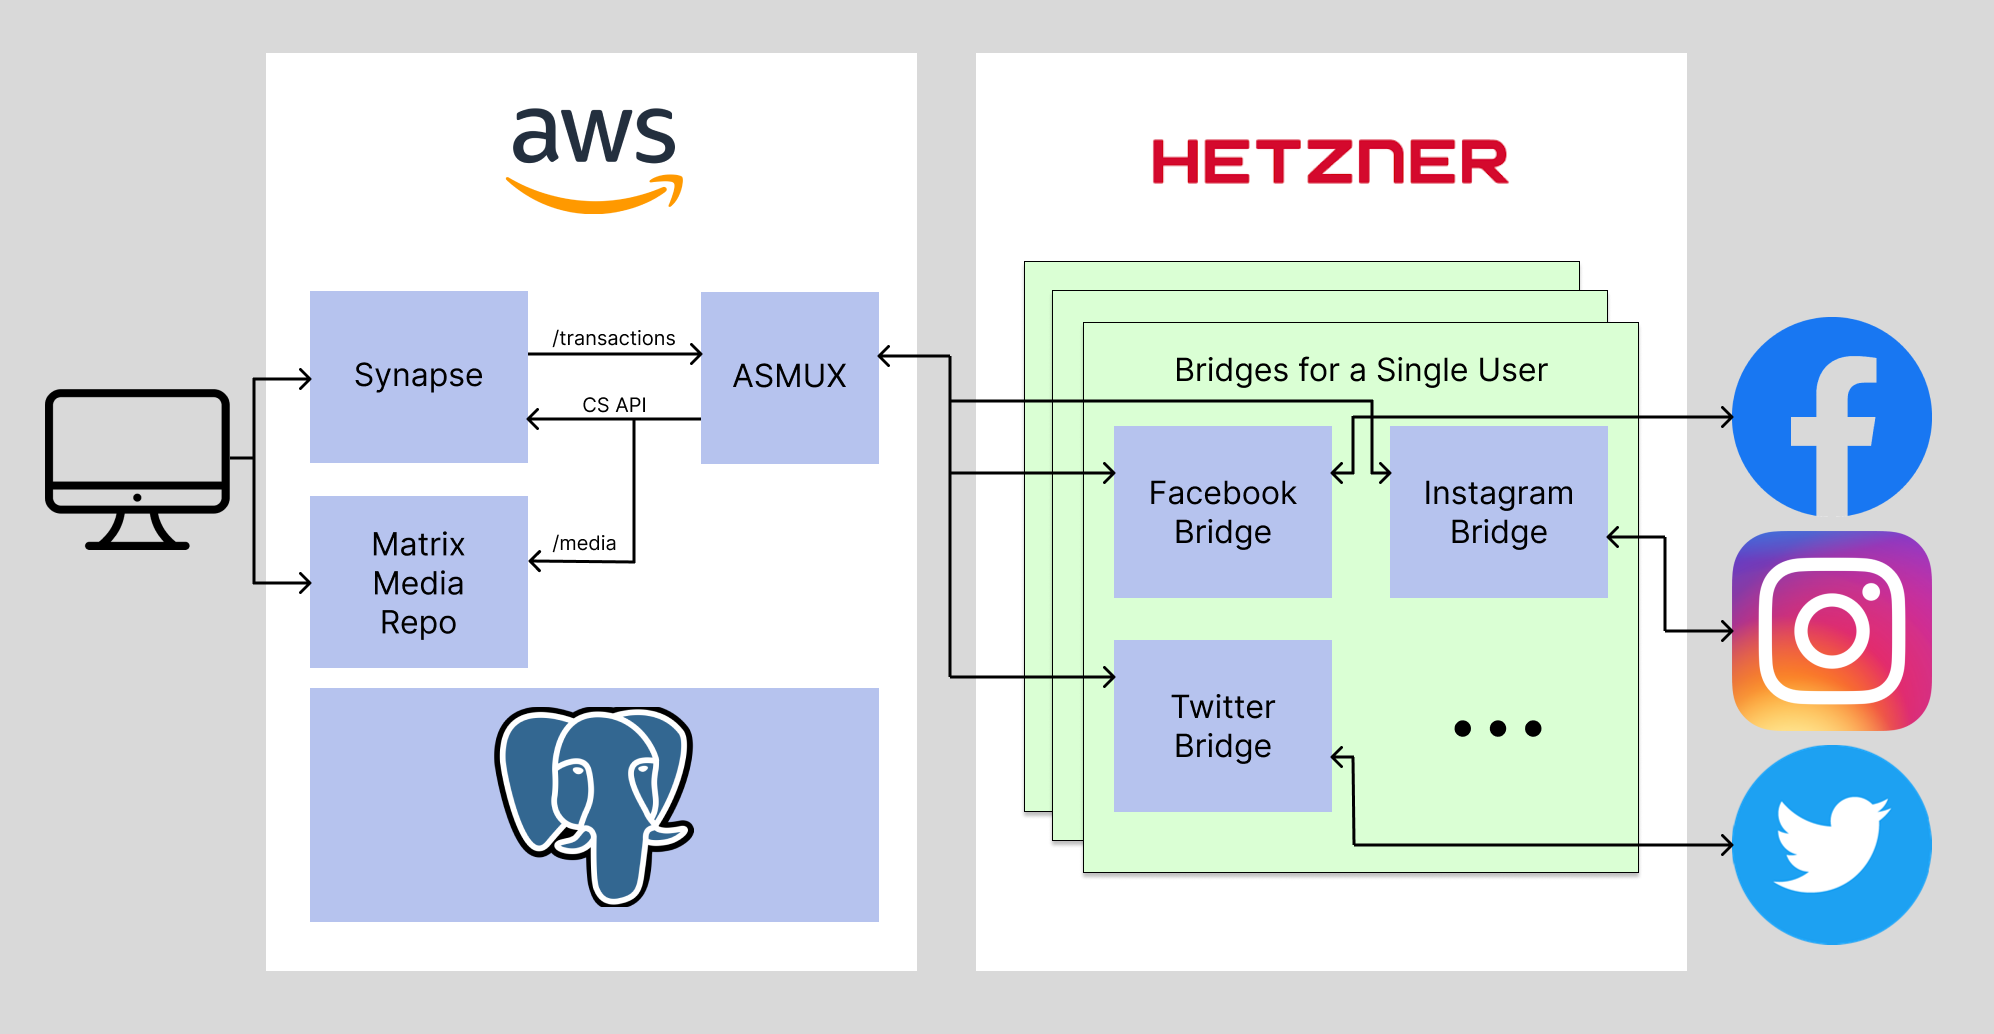
\includegraphics[width=1.15\textwidth]{images/current-architecture}}
    The core software in this architecture is Synapse.
\end{frame}

\begin{frame}{Stats}
    Because we encourage users to connect every chat network, we have a lot of
    puppet users.

    \textbf{\large On average, each user brings 4716 puppeted users.}
    \vspace{0.4cm}
    \pause

    All of these puppets represent real people on other networks, so they
    each generate their own traffic.

    \textbf{\large On average, each user and their puppets collectively account
        for 100k events!}
    \vspace{0.4cm}
    \pause

    None of that traffic is federated, but it has to go to Synapse which is
    designed with federation front-and-center!
\end{frame}

\begin{frame}{A few more notes}
    \begin{itemize}[<+->]
        \item \textbf{Synapse is aggressively federated}

            Synapse has no special handling of federated vs unfederated rooms.

        \item \textbf{Synapse does not handle message floods well}

            Synapse falls over when users bridge some large Telegram chats and
            Discord servers.

        \item \textbf{Deleting rooms from Synapse is hard}

            We end up with lots of \textit{dead} rooms when users delete their
            bridges and never turn it back on (or need a hard bridge reset).
    \end{itemize}
\end{frame}

\begingroup
\def\insertframenumber{\relax}
\begin{frame}[standout]
    \Large
    Solution: shard our homeserver based on bridged vs. unbridged traffic
\end{frame}
\endgroup

\section{Our new architecture}

\begin{frame}{A sharded future}
    \centerline{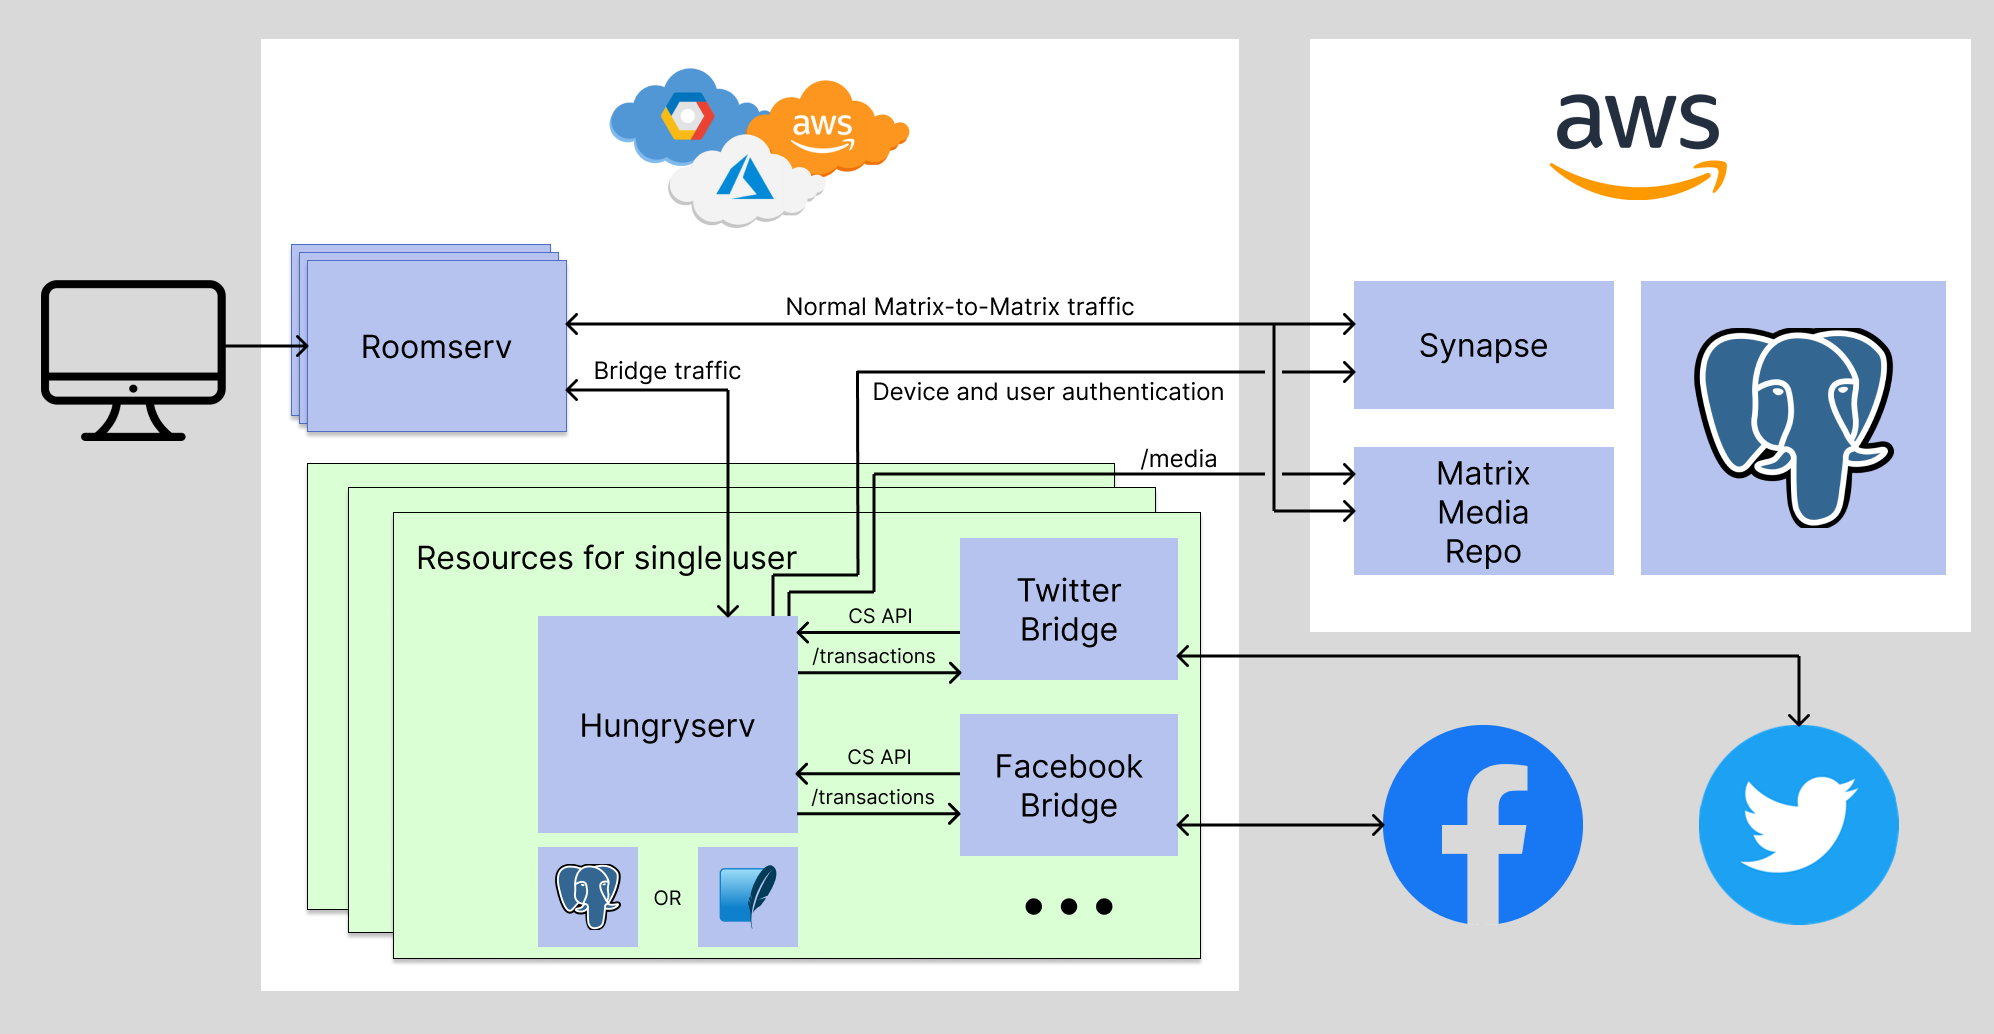
\includegraphics[width=1.15\textwidth]{images/new-architecture}}

    Let's talk about the differences from the old architecture\ldots
\end{frame}

\begin{frame}{Splitting the homeserver, keeping the protocol}
    \Large
    \centering
    This new architecture allows us to handle Matrix-native federated traffic
    separately from our high-throughput unfederated bridge traffic.
    \pause

    \textbf{All while maintaining API compatibility with clients, bridges, and
    the Matrix federation!}
\end{frame}

\begin{frame}{A sharded future}
    \centerline{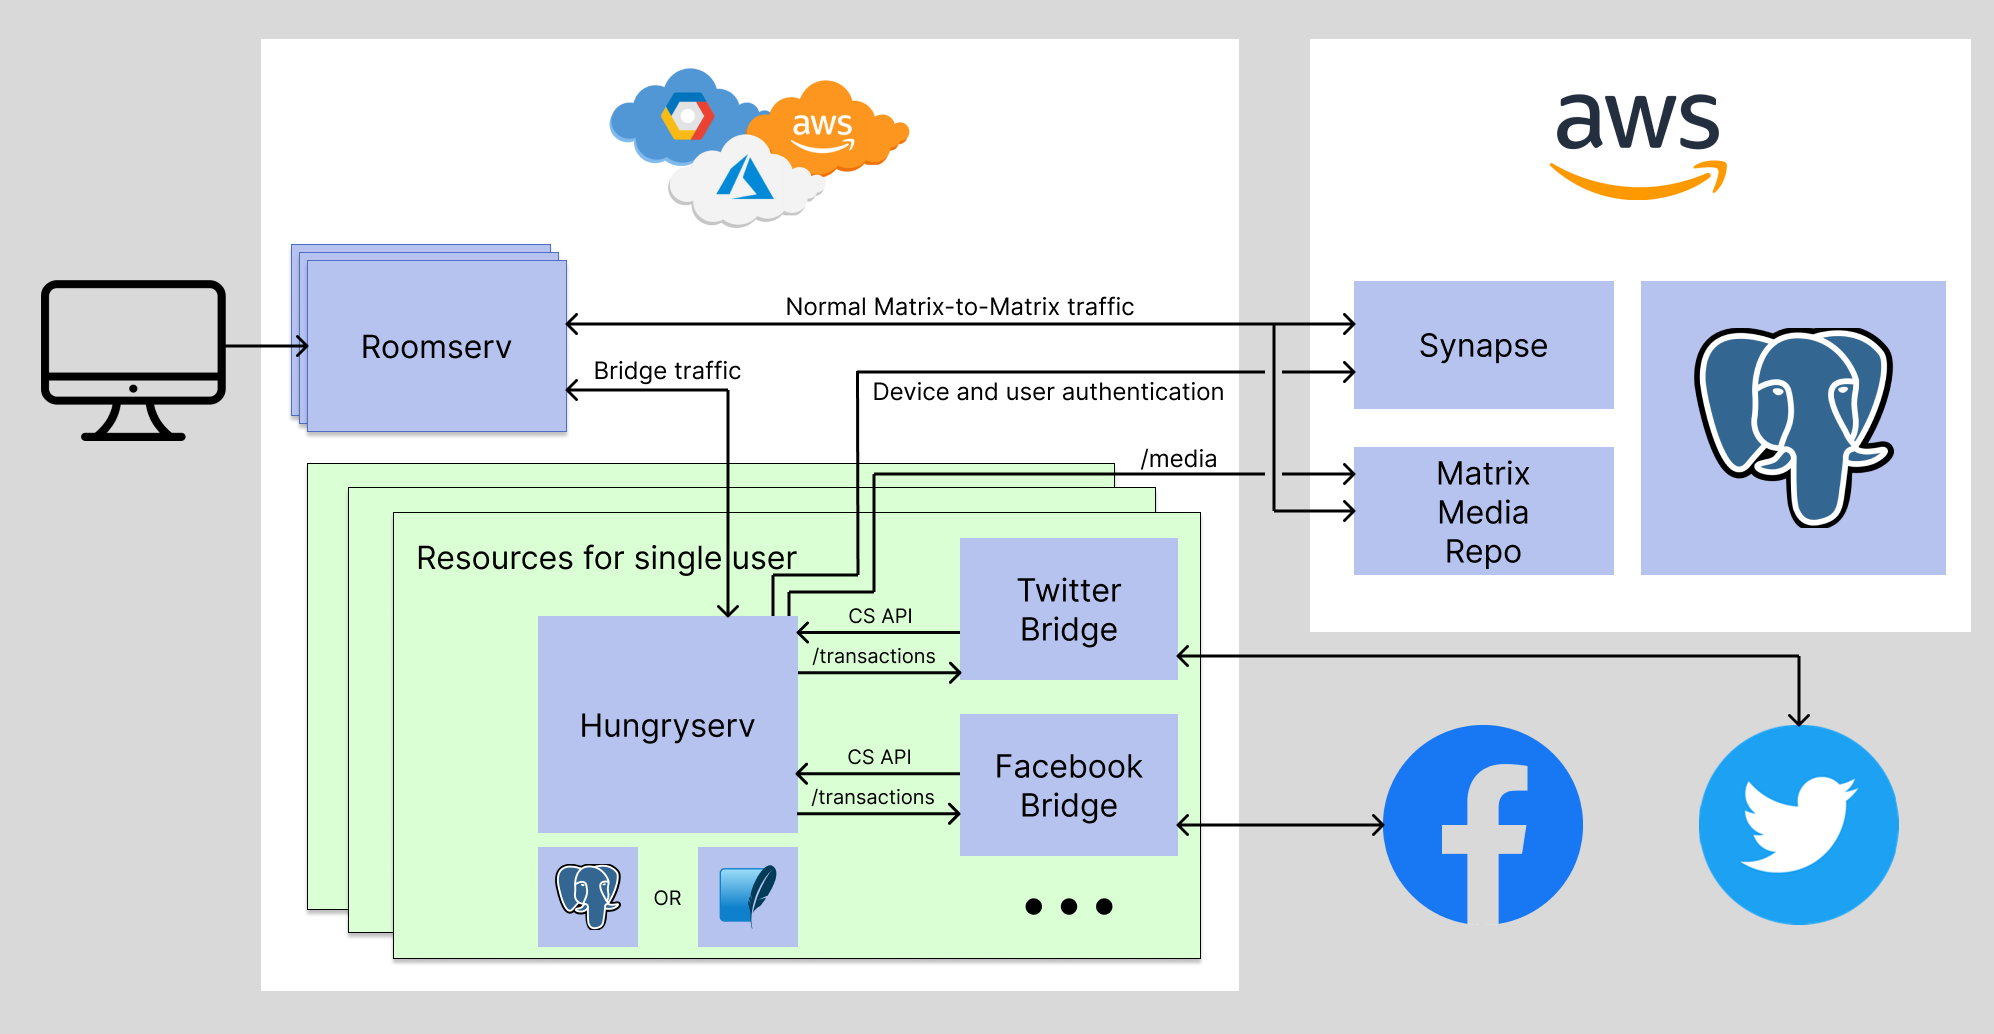
\includegraphics[width=1.15\textwidth]{images/new-architecture}}

    Let's talk about the differences from the old architecture\ldots
\end{frame}

\begin{frame}{Hungryserv: why is it hungry?}
    \Large
    Because it's unfed\pause{erated!}
\end{frame}

\begin{frame}{Hungryserv}
    We run a \textbf{Hungryserv} instance for every user to handle that user's
    bridge traffic.
    \pause

    \begin{itemize}[<+->]
        \item If there's a message flood from a bridge, it only affects that
            user.
        \item We don't have to store all of the bridge events and users in our
            Synapse database.
        \item Synapse is less resource constrained and can do what it does best:
            federate with other Matrix homeservers.
    \end{itemize}
    \pause[\thebeamerpauses]

    We are also currently looking into ways of using \textbf{SQLite} in
    production using Litestream.
\end{frame}

\begin{frame}{Hungryserv: aggressively unfederated}
    Each bridge belongs to a single user, so federation is unnecessary. \\
    \pause

    \begin{quote}
        When your DAG is a linked-list, don't store it as a DAG.
    \end{quote}
    \pause

    Being unfederated means that:
    \begin{itemize}
        \item we can avoid implementing the state resolution algorithm,
        \item event storage requires less metadata,
        \item deletions can be optimized, and
        \item infinite backfill becomes an simple batch SQL operation.
    \end{itemize}
\end{frame}

\begin{frame}{Hungryserv: goals, and non-goals}
    \textbf{Goals}
    \begin{itemize}
        \item Be fast
        \item Be compatible with Beeper clients (and mostly compatible with
            Element clients)
        \item Be API-compatible with the Appservice API for bridges
    \end{itemize}
    \pause

    \textbf{Non-goals}
    \begin{itemize}
        \item Be federated
        \item Be fully spec compliant
    \end{itemize}
\end{frame}

\begin{frame}{A sharded future}
    \centerline{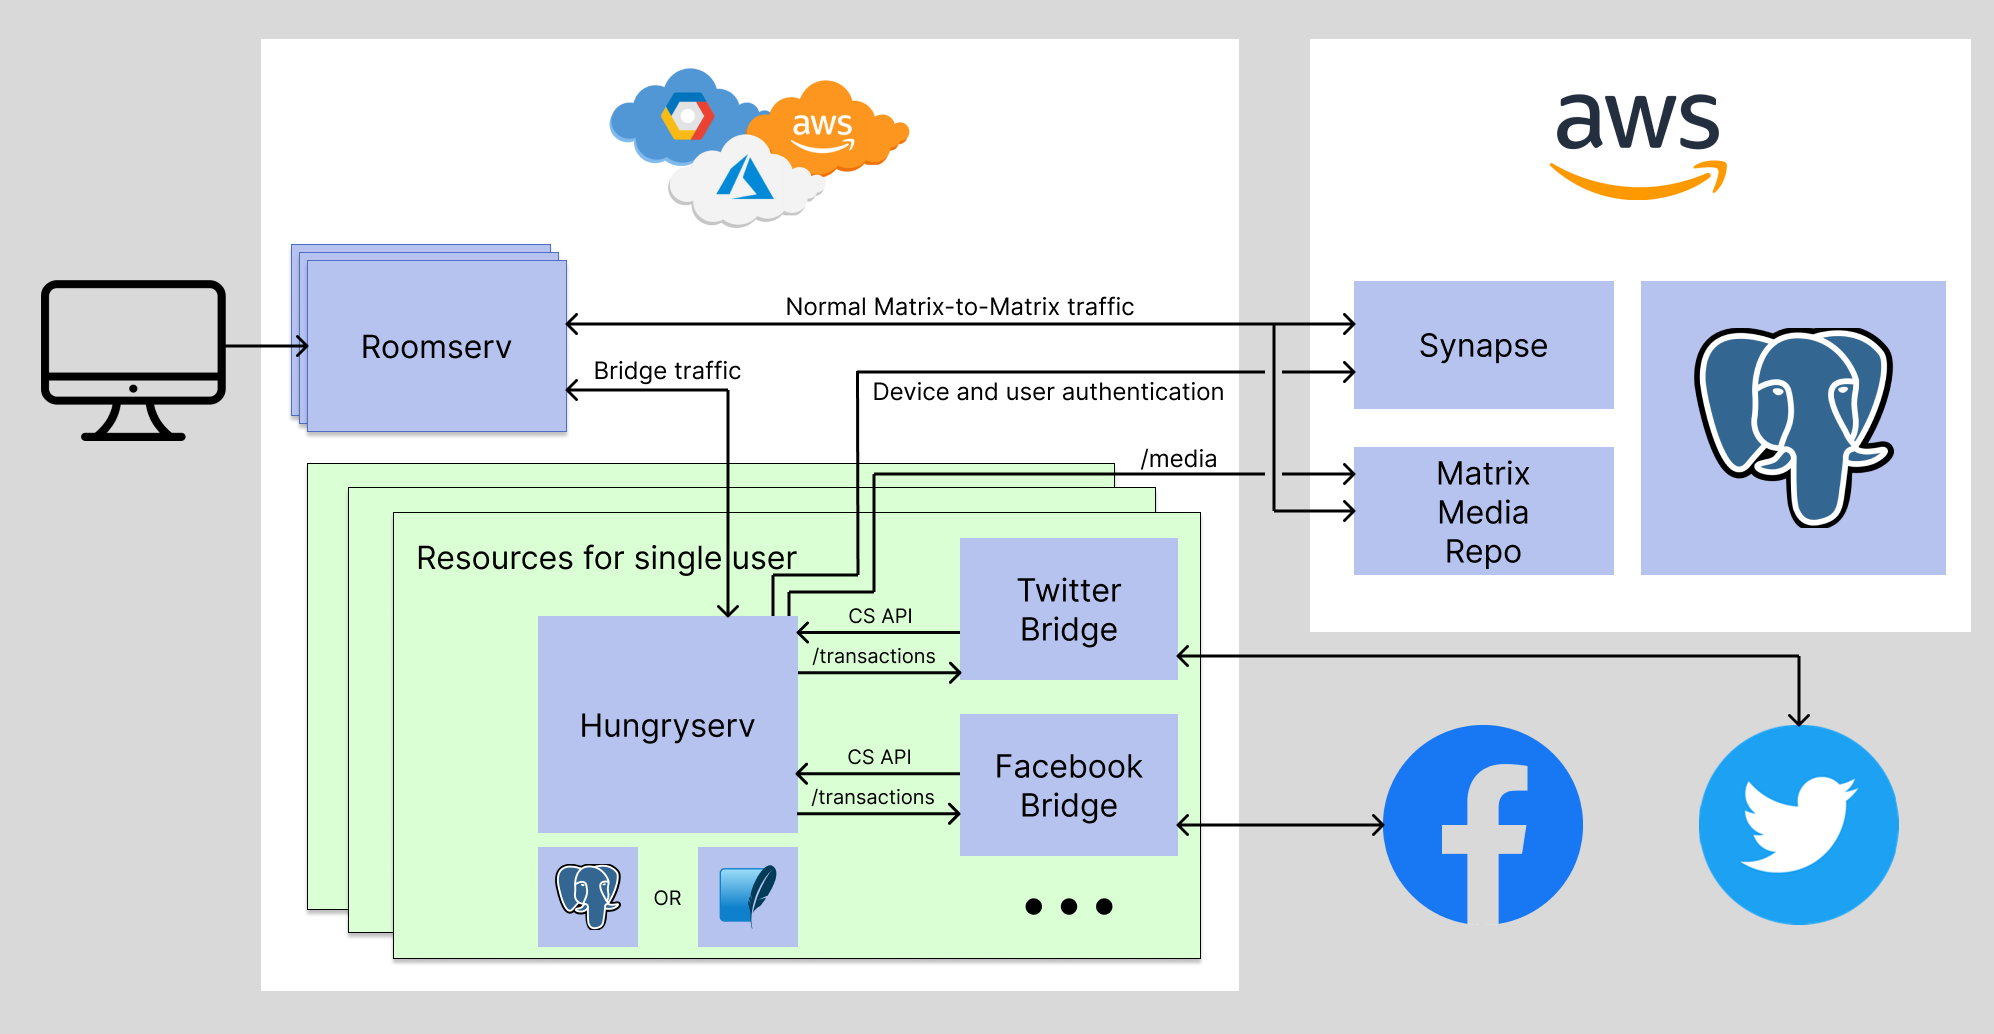
\includegraphics[width=1.15\textwidth]{images/new-architecture}}

    Let's talk about the differences from the old architecture\ldots
\end{frame}

\begin{frame}{Roomserv}
    \textbf{Roomserv} is a service which splits client requests between Synapse
    and Hungryserv.

    Roomserv merges the responses from the two homeservers to make it appear as
    a single homeserver to the client.
\end{frame}

\begin{frame}{A sharded future}
    \centerline{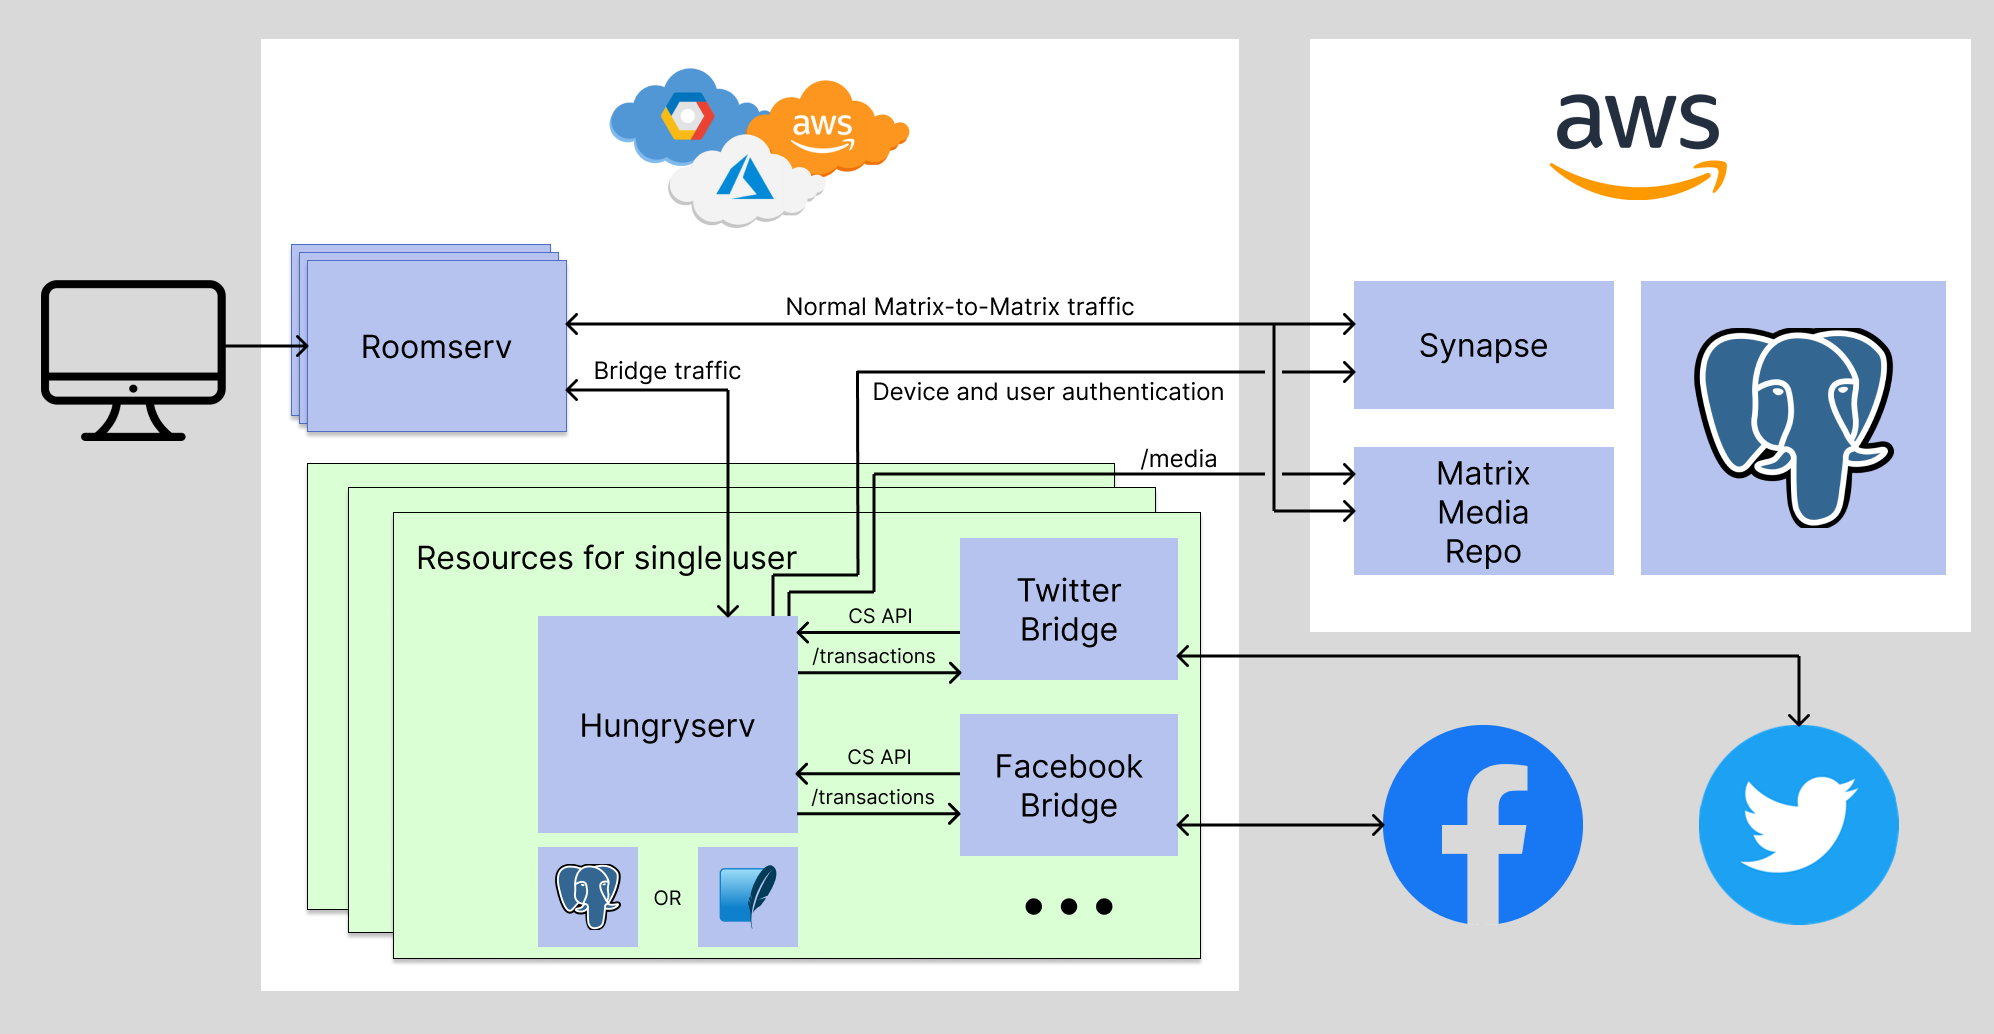
\includegraphics[width=1.15\textwidth]{images/new-architecture}}

    Let's talk about the differences from the old architecture\ldots
\end{frame}

\begin{frame}{No more ASMUX}
    Hungryserv natively supports dynamic registration of app services, and knows
    how to route requests to the correct bridge.
    \pause

    \textbf{We no longer have to rely on the single transactions firehose from
    Synapse.}
\end{frame}

\begin{frame}{A sharded future}
    \centerline{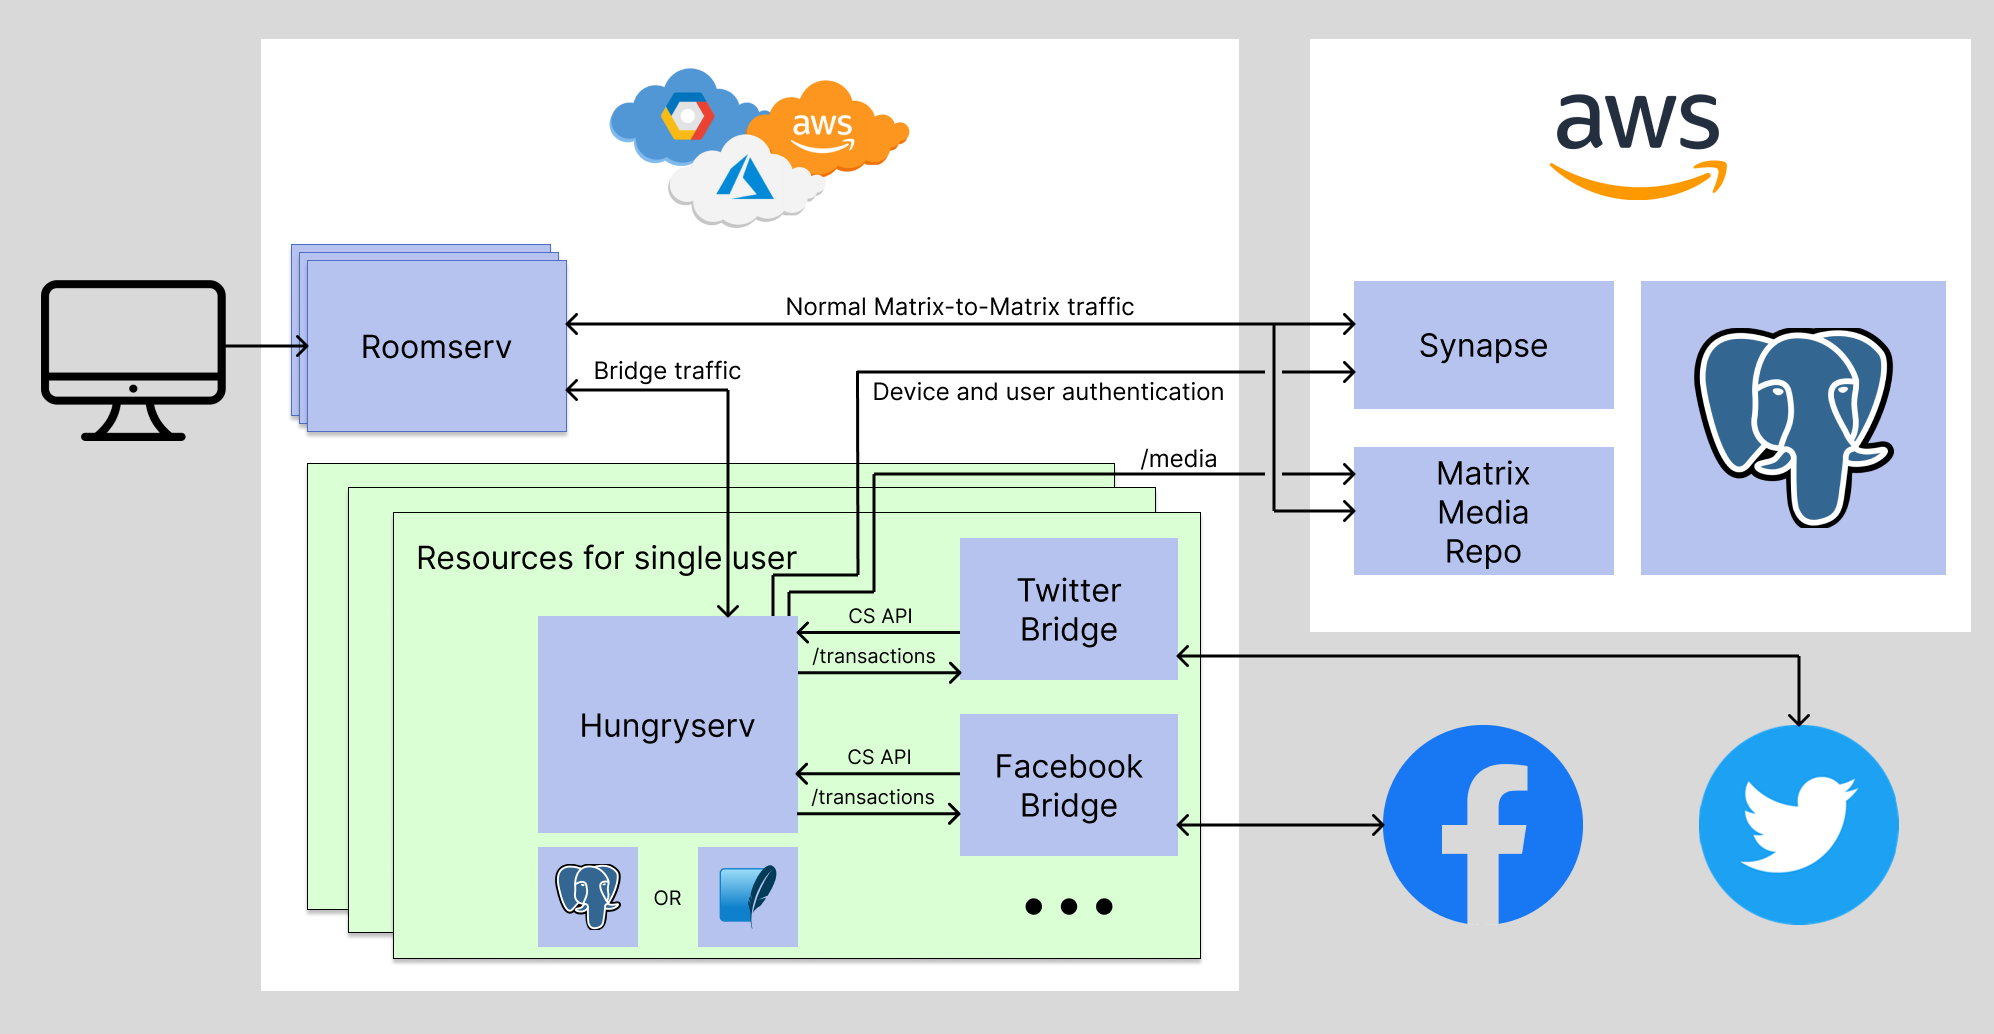
\includegraphics[width=1.15\textwidth]{images/new-architecture}}

    Let's talk about the differences from the old architecture\ldots
\end{frame}

\begin{frame}{A multi-cloud future?}
    The resources for each user can be moved closer to them using a multi-cloud,
    or multi-region strategy.

    This will help reduce latency (especially to bridged networks) and allow for
    us to deploy in more flexible and cost-effective environments.
\end{frame}

\begin{frame}{A sharded future}
    \centerline{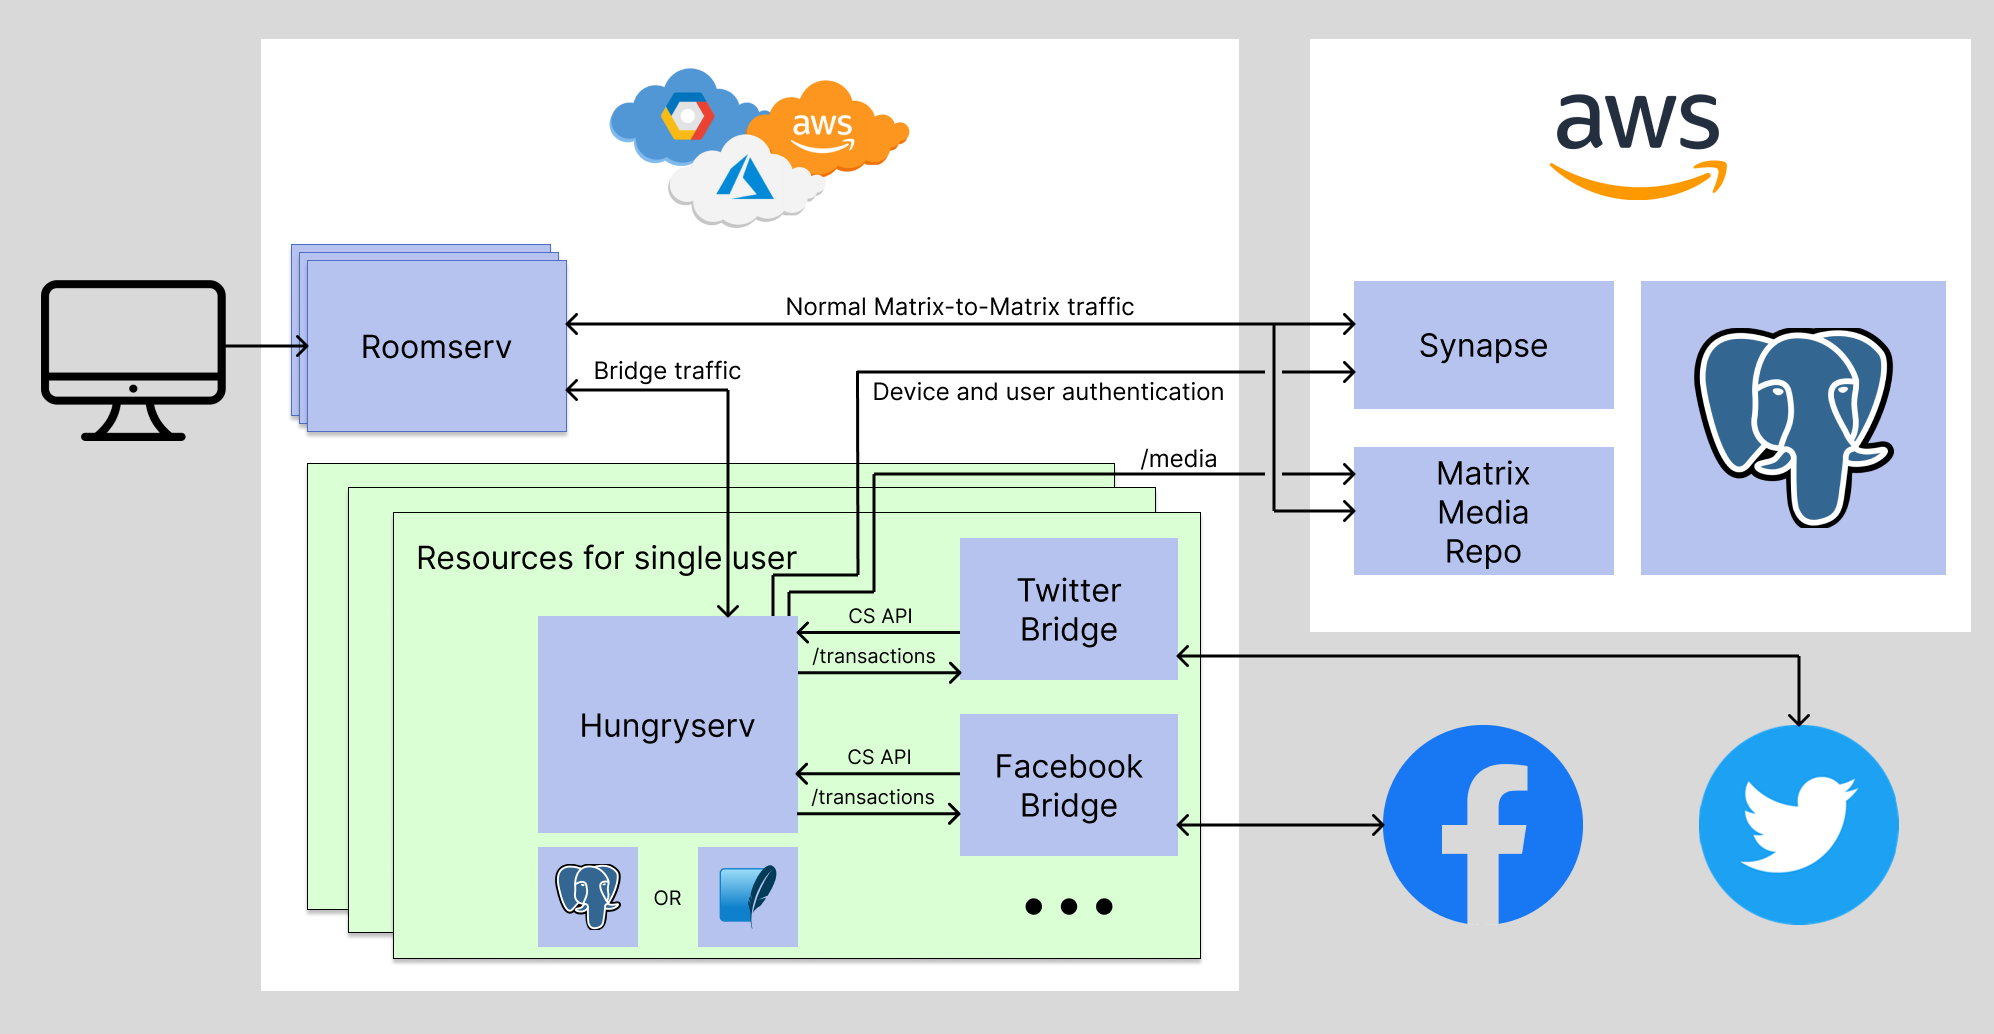
\includegraphics[width=1.15\textwidth]{images/new-architecture}}

    Let's talk about the differences from the old architecture\ldots
\end{frame}

\begingroup
\def\insertframenumber{\relax}
\begin{frame}[standout]
    \Large
    Demo!
\end{frame}

\begin{frame}[standout]
    \Large
    Questions?
\end{frame}
\endgroup

\end{document}
% Local Variables:
% TeX-command-extra-options: "-shell-escape"
% End:
